\section{Exploración de datos}

En primer lugar, tras descargar los distintos conjuntos de imágenes pasamos a analizar simplemente el balanceo entre las clases. Nos encontramos antes un problema de clasificación de imágenes y en un campo como es el de la oncología en el que no tenemos experiencia ninguna, por tanto no podemos hacer un análisis mucho más extenso que éste. Al fin y al cabo lo que buscamos entrenando distintas redes neuronales es que sean estas, con su capacidad de aprendizaje, las que nos ayuden a determinar y extraer las características más relevantes de las imágenes para la clasificación que nos ocupa. En la siguiente se muestra un histograma con el número de imágenes de cada clase, además se ha diferenciado entre las imágenes del conjunto base y las imágenes adicionales que se proporcionan en la misma plataforma para contar con más ejemplos que nos ayuden a entrenar nuestras redes (de este modo podemos ver como el desbalanceo es similar en ambos conjuntos de imágenes):\\

\begin{figure}[H]
  \centering
  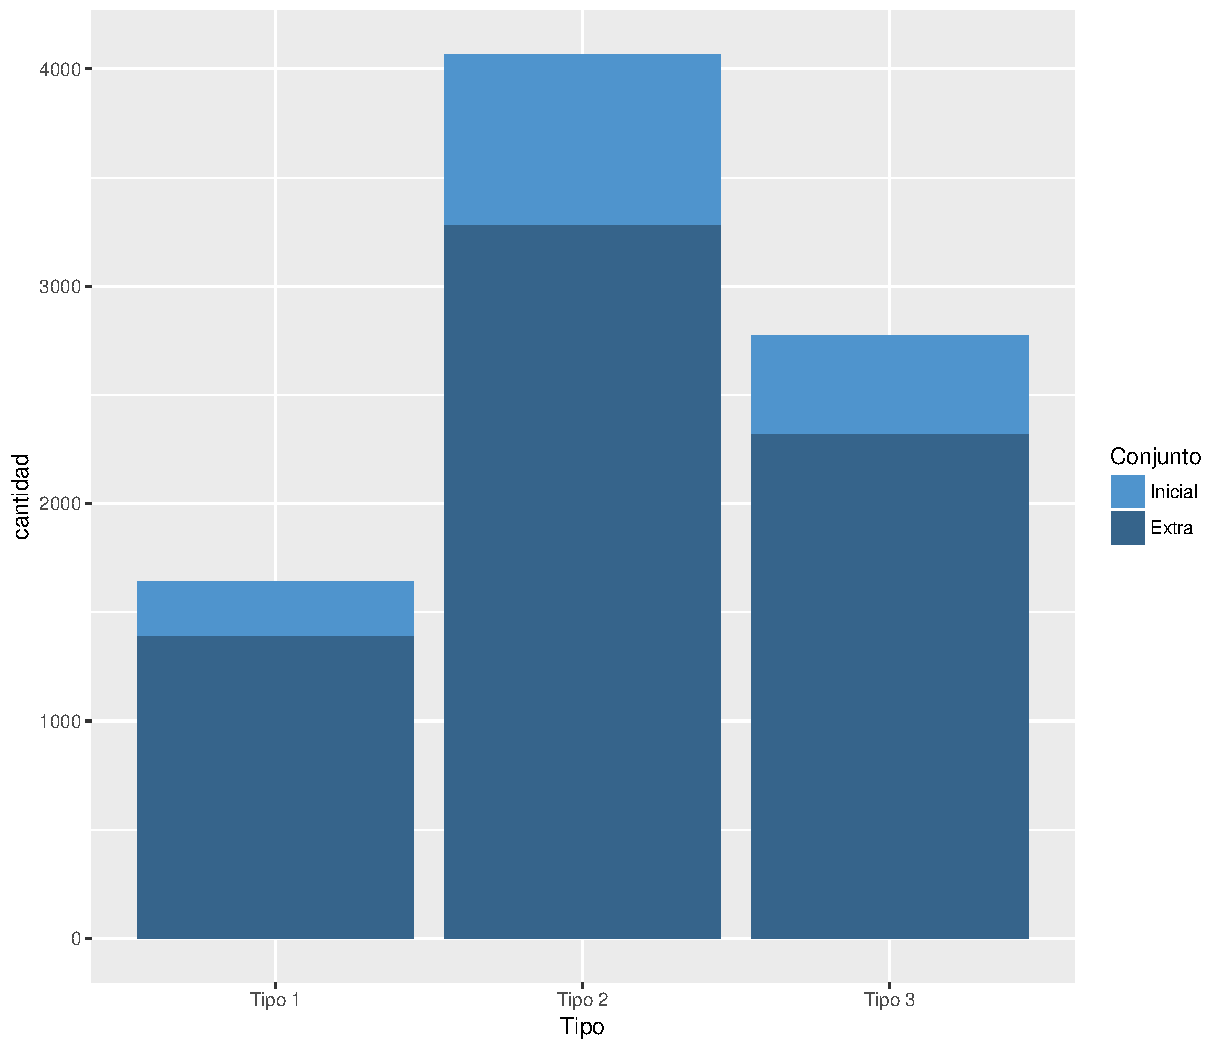
\includegraphics[scale=0.5]{img/conteo.pdf}
  \caption{Desbalanceo entre clases}
\end{figure}

Como podemos ver las clases presentar un cierto desbalanceo, siendo el cáncer tipo 2 del que más muestras disponemos. Con lo cual estaríamos trabajando en un problema desbalanceado, no obstante en esta práctica no se a tratado este problema por falta de tiempo, quedando el balanceo de las clases como trabajo futuro.\\
 
Por la poca experiencia con la que contamos en el campo esta es la escasa exploración de datos que se ha podido realizar, pasamos a hablar del procesamiento realizado sobre nuestras imágenes.
